\documentclass{article}
\usepackage[utf8]{inputenc}
\usepackage{amsmath}
\usepackage{amssymb}
\usepackage{graphicx}

\graphicspath{{Images/}}


\setlength{\oddsidemargin}{0in}
\setlength{\textwidth}{6.5in}
\setlength{\topmargin}{-.55in}
\setlength{\textheight}{9in}
\pagestyle{empty}


\title{Solid State Physics HW3}
\author{Michael Nameika}
\date{September 2022}

\begin{document}

\maketitle
To begin, recall Bragg's Law:
\begin{equation}
    n\lambda = 2d\sin{(\theta)}
\end{equation}
and the formula that relates distance to $hkl$:
\begin{equation} 
    d^2 = \frac{a^2}{h^2 + k^2 + l^2}
\end{equation}
That is, $1/d^2$ is an integer multiple of $1/a^2$, which we may use to solve for $a$. Additionally, for our use, we will assume $n = 1$ in Bragg's law.
\section*{Problem 1}
a) Plotting the second column as a function of the first in MATLAB, we find the following plot:
\begin{center}
    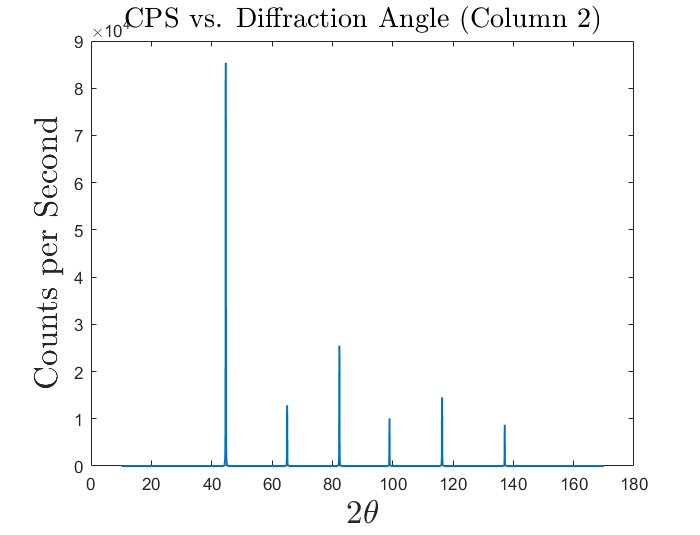
\includegraphics[scale = 0.75]{column2.png}
\end{center}

b) After calculating $d$ from Bragg's law for each of the peaks (see table below), we notice that the smallest distance between values of $1/d^2$ is $0.2420903$, which leads us to a lattice constant of $a = 2.03241$, with a miller index of the first plane of diffraction of (100), a property that no material possesses. Thus, we must now consider the case where the first Miller index is (110). As we will see, doing so will lead us to a material that exists.
\begin{center}
    \begin{tabular}{c|c|c|c|c|c}
        $i$ & $2\theta$ & $d\: [\text{\AA}]$ & $1/d^2\: [\text{\AA}^{-2}]$  & ratio to 0.1210452 & $(hkl)$ \\
        \hline
        1 & $44.65^{\circ}$ & 2.03241 & 0.2420903 & 2 & (110)\\
        2 & $65^{\circ}$ & 1.4368704 & 0.4843561 & 4 & (200)\\
        3 & $82.35^{\circ}$ & 1.17265 & 0.72721559 & 6 & (211)\\
        4 & $98.95^{\circ}$ & 1.01567 & 0.9693816 & 8 & (220)\\
        5 & $116.4^{\circ}$ & 0.908385 & 1.2118813 & 10 & (310)\\
        6 & $137.15^{\circ}$ & 0.82934 & 1.4539008 & 12 & (222)\\
    \end{tabular}
\end{center}
The last column of the above table can be found by solving the Diophantine equation $h_i^2 + k_i^2 + l_i^2 = n_i$, where $n$ denotes the ratio of $1/d^2$ to 0.1210452. Seeing as how the Miller indices are strictly even numbers, it is a fair assumption that this material is in the base centered cubic system. 
\newline

c) Since the ratio between $1/d_1^2$ and 0.2420903 is two, we can see that the smallest gap between diffraction planes is $0.1210452$. Then it is natural to assume $1/a^2 = 0.1210452$ by equation (2), so $a = 2.8743 \text{\AA}$.
\newline

d) Upon inspection of table 3 in Kittel, we can see that iron (Fe) crystallizes in the base centered cubic system and has lattice constant of $2.87 \text{\AA}$. Thus, I believe that the most probable material given this data is iron.


\section*{Problem 2}
e) Plotting the third column as a function of the first, we find
\begin{center}
    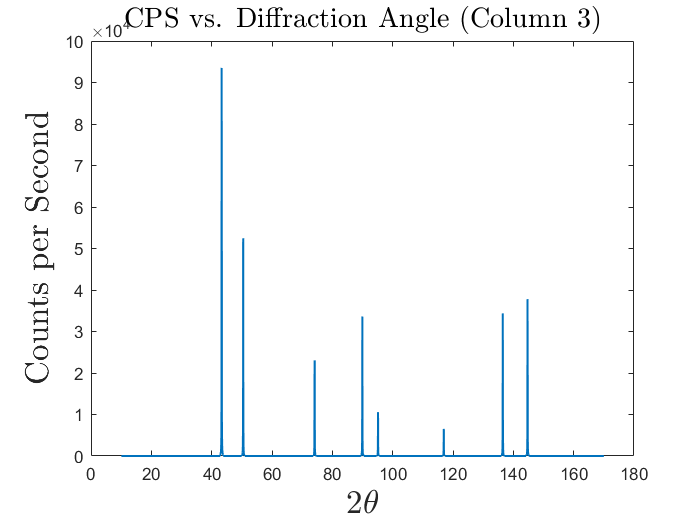
\includegraphics[scale = 0.75]{column3.png}
\end{center}

f) Inspecting the peaks of the graphs and using (1) and noticing that the smallest difference between $1/d^2$ terms is 0.076698, we find 
\begin{center}
    \begin{tabular}{c|c|c|c|c|c}
        $i$ & $2\theta$ & $d\: [\text{\AA}]$ & $1/d^2\: [\text{\AA}^{-2}]$  & ratio to 0.076698 & $(hkl)$\\
        \hline
        1 & $43.3^{\circ}$ & $2.08789$ & $0.229395$ & $3$ & (111)\\
        2 & $50.45^{\circ}$ & $1.80748$ & $0.306093$ & $4$ & (200)\\
        3 & $74.15^{\circ}$ & $1.27774$ & $0.612513$ & $8$ & (220)\\
        4 & $89.89^{\circ}$ & $1.08984$ & $0.841927$ & $11$ & (311)\\
        5 & $95.15^{\circ}$ & $1.04354$ & $0.918294$ & $12$ & (321)\\
        6 & $116.95^{\circ}$ & $0.903670$ & $1.224561$ & $16$ & (400)\\
        7 & $136.5^{\circ}$ & $0.829340$ & $1.453901$ & $19$ & (331)\\
        8 & $144.7^{\circ}$ & $0.808351$ & $1.530383$ & $20$ & (442)\\
    \end{tabular}
\end{center}
Notice that the Miller indices in the above table satisfy the restrictions for face centered cubic, so it is safe to assume that the material crystalizes in the face centered cubic structure.
\newline

g) Since $0.076698$ is the smallest difference between values of $1/d^2$, it is natural to assume $1/a^2 = 0.076698$ by equation (2), or alternatively, $a = 3.61084 \text{\AA}$.
\newline

h) Using Table 3 in Kittel, we can see that copper (Cu) is face centered cubic with a lattice parameter of $3.61 \text{\AA}$, matching the values we found from this plot. Thus, I believe that Copper is the most probable material given this data.





\section*{Problem 3}
i) Plotting the fourth column as a function of the first, we find
\begin{center}
    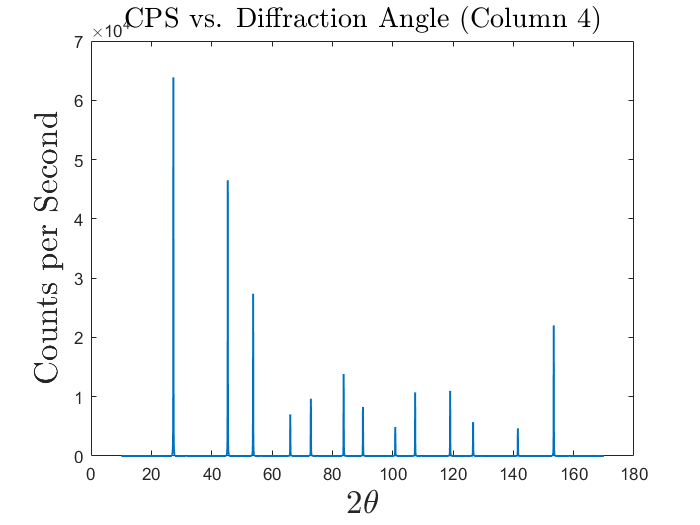
\includegraphics[scale = 0.75]{column4.png}
\end{center}

j) Calculating $d$ by using (1) and noticing that the smallest difference between $1/d^2$ terms is given by $0.0938578$,we may also observe that $0.0938578$ does not evenly divide into most of the values of $1/d^2$. However, by inspection, it is clear to see that $0.0938578/3 = 0.0312859$ evenly divides each $1/d^2$.
\begin{center}
    \begin{tabular}{c|c|c|c|c|c}
        $i$ & $2\theta$ & $d\: [\text{\AA}]$ & $1/d^2\: [\text{\AA}^{-2}]$  & ratio to 0.0312859 & $(hkl)$\\
        \hline
         1 & $27.3^{\circ}$ & 3.26411 & 0.0938578 & 3 & (111) \\
         2 & $31.65^{\circ}$ & 1.26392 & 0.125329 & 4 & (200) \\
         3 & $45.35^{\circ}$ & 1.99816 & 0.2504606 & 8 & (220) \\
         4 & $53.75^{\circ}$ & 1.70403 & 0.34438603 & 11 & (311) \\
         5 & $66.05^{\circ}$ & 1.41338 & 0.50059 & 16 & (400) \\
         6 & $72.9^{\circ}$ & 1.29654 & 0.594878 & 19 & (331) \\
         7 & $75.1^{\circ}$ & 1.26392 & 0.6359805 & 20 & (420) \\
         8 & $83.75^{\circ}$ & 1.15399 & 0.7509239 & 24 & (422) \\
         9 & $90.15^{\circ}$ & 1.08794 & 0.84487 & 27 & (333) \\
         10 & $100.85^{\circ}$ & 0.999361 & 1.00128 & 32 & (440) \\
         11 & $107.45^{\circ}$ & 0.955485 & 1.095348 & 35 & (531) \\
         12 & $109.7^{\circ}$ & 0.942092 & 1.1267132 & 36 & (600) \\
         13 & $119.05^{\circ}$ & 0.893773 & 1.25183 & 40 & (620) \\
         14 & $126.65^{\circ}$ & 0.862049 & 1.34566 & 43 & (533) \\
         15 & $129.3^{\circ}$ & 0.852375 & 1.376381 & 44 & (622) \\
         16 & $141.5^{\circ}$ & 0.815918 & 1.502128 & 48 & (444) \\
         17 & $153.4^{\circ}$ & 0.791529 & 1.596123 & 51 & (551) \\
    \end{tabular}
\end{center}
Further notice that the Miller indices satisfy the face centered cubic restrictions, so it is a fair assumption that this substance has face centered cubic structure. Additionally, rows 2, 7, 12, and 15 correspond to peaks with low intensity. Then these bands are essentially "forbidden" and we are working with a compound rather than an element.
\newline

k) Seeing as 0.0312859 is the largest divisor for each $1/d^2$ in the above table, it is fair to assume that $1/a^2 = 0.0312859$ by equation (2), or alternatively, $a = 5.65361 \text{\AA}$
\newline

l) On page 18 of Kittel, we can see that gallium arsenide (GaAs) has a lattice parameter of $5.65 \text{\AA}$, and happens to be face centered cubic. Thus, I believe that gallium arsenide is the most probable material given this data.


\section*{Problem 4}

\textbf{\textit{Form factor of atomic hydrogen.}} For the hydrogen atom in its ground state, the number density is $n(r) = (\pi a_0^3)^{-1}\exp{(-2r/a_0)}$, where $a_0$ is the Bohr radius. Show that the form factor is $f_G = \frac{16}{(4 + G^2a_0^2)^2}$.
\newline

Proof: Recall the formula for finding the atomic form factor: 
\[f_j = 4\pi \int n_j(r)r^2\sin{(Gr)}(Gr)^{-1}dr\]
Plugging in the given equation for $n(r)$, our equation becomes
\[f = 4\pi \int_0^{\infty} r\sin{(Gr)}e^{-2r/a_0}(\pi a_0^3)^{-1} dr\]
Substituting $x = Gr$ into the above integral gives us
\[f = \frac{4}{G^3a_0^3} \int_0^{\infty} x\sin{(x)}e^{-2x/(Ga_0)} dx\]
Notice the above integral can be rewritten as
\[\frac{4}{G^3a_0^3} \int x\sin{(x)}e^{-2x/(Ga_0)} dx = \text{Im}\left\{ \frac{4}{G^3a_0^3}\int xe^{\left(i - \frac{2}{Ga_0}\right)x}dx \right\}\]
Solving the right hand side, integration by parts gives us the following:
\[\frac{4}{G^3a_0^3}\int xe^{\left(i - \frac{2}{Ga_0}\right)x} dx = -\frac{2Ga_0 + iG^2a_0^2}{Ga_0i - 2}xe^{-\frac{2}{Ga_0}x}[\cos{(x)} + i\sin{(x)}] - \frac{(2Ga_0 - iG^2a_0^2)^2}{(4 + G^2a_0^2)^2}e^{-\frac{2}{Ga_0}x}[\cos{(x)} + i\sin{(x)}] + C\]
where $C$ is a constant of integration. Using this, we have
\[\text{Im}\left\{\frac{4}{G^3a_0^3}\int_0^{\infty} xe^{\left(i - \frac{2}{Ga_0}\right)x} dx\right\} = 4\left( -\frac{e^{-\frac{2}{Ga_0}x}}{4 + G^2a_0^2}\left[ \left(G^2a_0^2x - \frac{1}{4+G^2a_0^2}4G^3a_0^3\right)\cos{(x)} + (2Ga_0x + 4G^2a_0^2)\sin{(x)} \right]\right)\bigg|_0^{\infty}\]
Evaluating, we find
\[\text{Im}\left\{\frac{4}{G^3a_0^3}\int_0^{\infty} xe^{\left(i - \frac{2}{Ga_0}\right)x}dx\right\} = \frac{16}{(4 + G^2a_0^2)^2}\]
which is what we wanted to show.


\end{document}
